\chapter{Évolution de PPanGGOLiN : présentation de la version 2}

PPanGGOLiN est un outil dont le développement a commencé (sur GitHub) en 2018. Avec plus de 2000 commits\footnote{ajout, suppression ou modification de code validé et marqué dans le système de gestion de version (ici Git)} actuellement, et 7 ans de développement, le code a connu de nombreuses évolutions. De plus, ces modifications sont l'\oe uvre de plusieurs développeurs qui se sont succédés et qui ont collaboré activement au projet.

Le développement de nouvelles méthodes, l'ajout de nouveaux outils, ou encore simplement le débogage devenaient de plus en plus lourds. De plus, dans le cadre de ma thèse, PPanGGOLiN allait être utilisé comme outil et certaines fonctionnalités devaient être améliorées. C'est avec cet objectif en tête que Jean Mainguy (ingénieur au LABGeM), Guillaume Gautreau (chercheur INRAE), Adelme Bazin (ingénieur de recherche), Alexandra Calteau (chercheuse CEA), David Vallenet (directeur de recherche CEA) et moi-même avons développé et proposé en janvier 2024 une version 2 de PPanGGOLiN. Cette nouvelle version contient de nouvelles fonctionnalités pour l'analyse des pangénomes, mais aussi de nombreuses améliorations techniques.

Dans ce chapitre, nous reviendrons sur les changements majeurs apportés dans la version 2 de PPanGGOLiN. D'autres changements plus anecdotiques ne seront pas abordés. Néanmoins, une des améliorations concerne l'écriture des notes de versions qui sont plus détaillées. Toutes les modifications sont alors visibles dans ces notes sur le GitHub de PPanGGOLiN \url{https://github.com/labgem/PPanGGOLiN/releases}.

\section{Nouvelles fonctionnalités et amélioration méthodologique}
\subsection{Developpement de nouvelles méthodes d’analyse}
\subsubsection{Recherche de contexte génomique}

\paragraph{Définition}

Le contexte génomique (\textit{Genomic Context}, GC) désigne l’organisation spécifique des gènes au sein d’un génome. Durant l'évolution, cette organisation va subir des pressions de sélection. Si elle se maintient conservée, on peut postuler que les gènes du GC sont impliqués dans un même processus biologique. C'est pourquoi, la recherche de GCs conservés dans les génomes est utilisée pour prédire la fonction de gènes inconnus en les associant à d'autres dont la fonction est connue. C'est le principe du coupable par association \cite{aravind_guilt_2000}. Rechercher un GC (ou un sous-ensemble de ce dernier) dans les génomes permet ainsi d'identifier des processus biologiques et des dérivés dans les génomes, comme le fait antiSMASH \cite{medema_antismash_2011}, en détectant spécifiquement les clusters de gènes biosynthétiques (BGCs).

\newpage

Une des méthodes de recherche de GC dans les génomes repose sur le voisinage des gènes dans les séquences. On considère des gènes comme fonctionnellement liés s’ils sont régulièrement retrouvés à proximité les uns des autres dans divers génomes, même sans être directement adjacents. Ce type de signal permet de détecter des associations fonctionnelles conservées, même entre des gènes non homologues. 

Cette approche est particulièrement intéressante dans le cadre des graphes de pangénome, comme ceux produits par PPanGGOLiN. Le graphe de pangénome intègre déjà l’information sur le voisinage direct des gènes à travers l’ensemble des génomes étudiés. Cela permet d’extraire efficacement le contexte génomique directement depuis le graphe. De plus, cette approche permet de capturer toute la diversité génomique d’un ensemble d’organismes : non seulement les gènes conservés dans toutes les souches, mais aussi les gènes accessoires, présents uniquement dans certaines d’entre elles. Ainsi, l’extraction du contexte génomique à partir d’un pangénome permet de mieux refléter la diversité biologique réelle tout en accélérant la prédiction fonctionnelle des gènes.

\paragraph{Méthode de recherche de contexte génomique}

L'algorithme de prédiction (\autoref{fig:searchCC}) s’inspire de celui proposé dans panModule \cite{bazin_panmodule_2021}. Cependant, contrairement à ce dernier, qui vise à extraire l’ensemble des contextes génomiques conservés, notre approche se focalise sur l’identification précise des contextes associés à un ensemble de protéines cibles. L’objectif est d’extraire, au sein du pangénome, les familles de gènes conservées dans le contexte de ces protéines.

La première étape consiste à aligner les gènes cibles (\textit{target}) avec les familles de gènes du pangénome. Cet alignement est effectué à l’aide de MMSeqs2 \cite{steinegger_mmseqs2_2017}, avec un seuil de 80 \% d'identité et 80 \% de couverture entre les séquences protéiques des gènes et celles des familles. Les familles correspondant aux séquences alignées sont alors étiquetées comme \textit{target} (représentées en bleu et orange dans la \autoref{fig:searchCC}).

\begin{figure}[htbp]
    \centering
    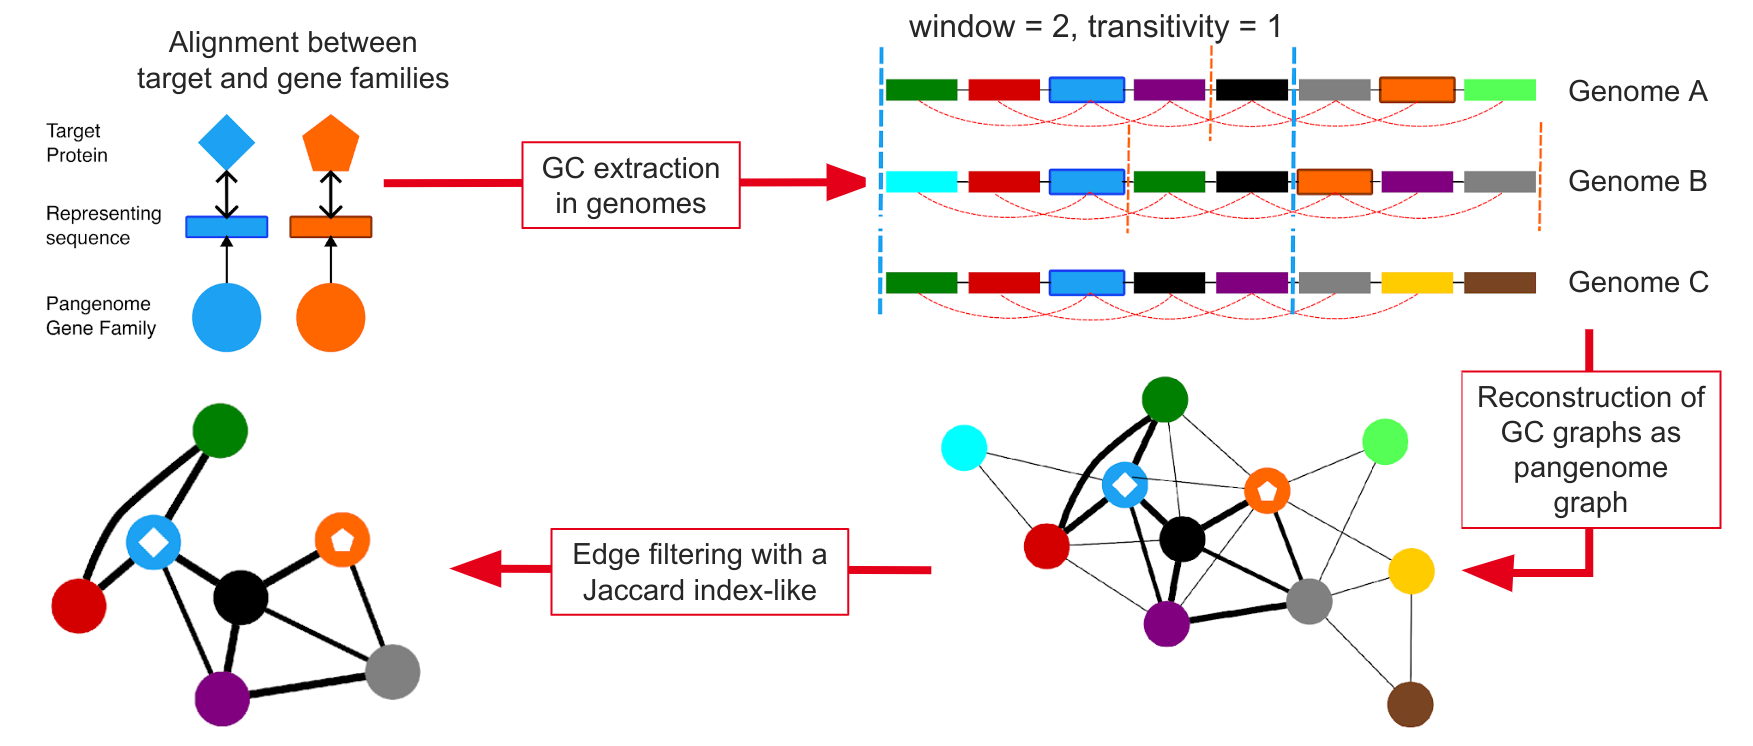
\includegraphics[width=\linewidth]{images/searchCC.png}
    \caption[Méthode de recherche du contexte génomique dans un graphe de pangénome]{\textbf{Méthode de recherche du contexte génomique dans un graphe de pangénome.}}
    \label{fig:searchCC}
\end{figure}

\newpage
À partir de ces familles \textit{target}, nous reconstruisons un sous-graphe du pangénome. Ce sous-graphe intègre non seulement les arêtes de voisinage direct, mais aussi des arêtes de transitivité reliant des familles situées à une distance $t$. Ainsi, l’algorithme capture non seulement les relations directes, mais aussi celles entre familles avoisinantes. Par exemple, dans la \autoref{fig:searchCC}, avec $t=1$, des arêtes de transitivité sont créées entre le gène bleu et les gènes vert et noir, ainsi qu'entre le gène violet et les gènes rouge et gris.

Pour limiter la taille du sous-graphe, un paramètre \textit{window} est introduit. Il contrôle le nombre de gènes adjacents — de part et d'autre de la \textit{target} — pris en compte pour la création des arêtes de transitivité.

Le sous-graphe obtenu forme alors une composante connexe intégrant l’ensemble des relations de voisinage jusqu’à la distance $t$. Un filtre de Jaccard (cf. \autoref{eq:jaccard}) est ensuite appliqué pour conserver uniquement les arêtes les plus pertinentes.

Enfin, nous extrayons toutes les composantes connexes contenant au moins une famille \textit{target}, représentant ainsi les contextes génomiques conservés autour des protéines cibles.

\subsubsection{Metadonnées}

Dans le cadre de l'ajout de nouvelles fonctionnalités à PPanGGOLiN, une première avancée que j'ai développée concerne l'ajout de \textbf{métadonnées} à l'ensemble des éléments du pangénome, incluant les gènes, contigs, génomes, familles, arêtes, RGPs, spots et modules. Le format attendu des métadonnées est particulièrement flexible, l'utilisateur fournit un fichier tabulé, ne nécessitant au minimum que l'identifiant de l'objet concerné dans le pangénome.  L’utilisateur peut ainsi associer des métadonnées de tout type, sans restriction de format. De plus, chaque métadonnée est liée à une source spécifique, ce qui permet à un même objet d’en contenir plusieurs, issues de différentes sources d’annotation. Pour assurer une gestion optimisée et performante, ces métadonnées sont directement enregistrées dans le fichier HDF5 du pangénome. Bien qu'elles ne soient pas directement exploitées pour l'analyse du pangénome, elles sont intégrées aux sorties générées par PPanGGOLiN afin de faciliter l'interprétation et l'exploration des résultats.

\subsubsection{Projection}

Pour faciliter l'exploration des résultats, une \textbf{nouvelle sortie de visualisation des données} a été développée en collaboration avec Jean Mainguy. Celle-ci permet de générer, pour chaque génome, un fichier JSON compatible avec Proksee \cite{grant_proksee_2023}. Grâce à cette fonctionnalité, il est désormais possible de visualiser un génome, sous forme circulaire (\autoref{fig:projection}), où les éléments du pangénome ont été intégrés, notamment les parties persistantes et variables, ainsi que les RGPs, spots et modules. Proksee permet également de lancer des analyses supplémentaires sur les génomes, comme CARD \cite{alcock_card_2023} pour annoter les gènes de résistance aux antibiotiques, CRISPRCasFinder \cite{couvin_crisprcasfinder_2018} pour la prédiction des systèmes CRISPR-Cas, ou encore Phigaro \cite{starikova_phigaro_2020} qui permet d'identifier les régions de prophages. 

\newpage
L'intégration de cette nouvelle sortie est d'autant plus intéressante dans une autre nouvelle fonctionnalité de PPanGGOLiN : la \textbf{projection} des résultats du pangénome sur un génome externe. En effet, il est désormais possible de comparer un nouveau génome au pangénome déjà calculé. Pour cela, les gènes du génome externe sont alignés aux séquences référentes des familles de gènes en utilisant MMSeqs2 \cite{steinegger_mmseqs2_2017}. Les gènes dont l'alignement dépasse un seuil défini d'identité et de couverture sont alors associés à une famille existante, tandis que les autres gènes forment chacun une nouvelle famille (singleton) attribuée à la partition du \textit{cloud}. Ainsi, l’ensemble des gènes du génome externe se voit assigner une partition, ce qui permet d’appliquer les algorithmes de prédiction des RGPs et d’associer les spots et les modules au génome étudié.

Enfin, cette fonctionnalité de projection prend également en compte les métadonnées, assurant ainsi la transmission des informations du pangénome aux gènes du génome externe. Cette intégration renforce la cohérence des analyses en permettant d’exploiter les annotations des utilisateurs pour une meilleure interprétation des résultats.

\begin{figure}[htbp]
    \centering
    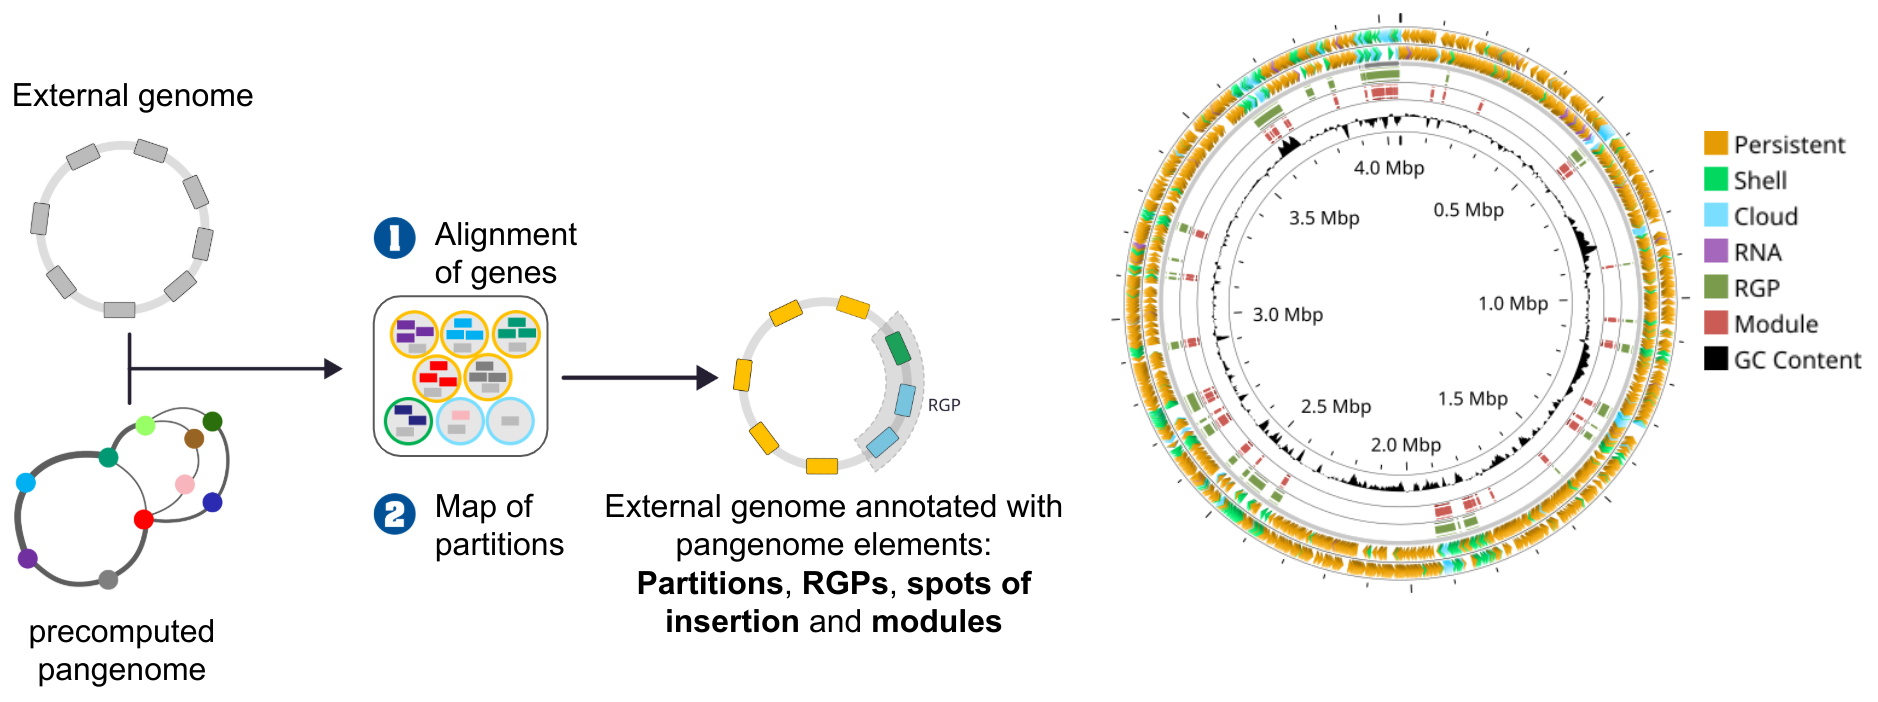
\includegraphics[width=\linewidth]{images/projection.png}
    \caption[Principe de fonctionnement de la méthode de projection]{\textbf{Principe de fonctionnement de la méthode de projection.} Le génome sur lequel le pangénome est projeté, est un génome de la même espèce que ceux qui ont servi à construire le pangénome. Sur la droite, un exemple de sortie disponible dans PPanGGOLiN et généré dans les projections, le Proksee \cite{grant_proksee_2023} d'un génome de \textit{A. baumannii} où les résultats du pangénome ont été projeté.}
    \label{fig:projection}
\end{figure}

\subsubsection{Analyse comparée des RGPs}

Une nouvelle fonctionnalité a été intégrée à PPanGGOLiN pour permettre l’analyse comparative des RGPs entre plusieurs génomes d’un même pangénome. Désormais, il est possible de regrouper (clusteriser) les RGPs similaires  (\autoref{fig:rgpcluster_met}). Deux RGPs sont considérés comme partageant un contenu commun si leurs gènes appartiennent aux mêmes familles de gènes. À partir de cette définition, un score de correspondance du répertoire génique (\textit{Gene Repertoire Relatedness}, GRR) est calculé, soit sur la RGP la plus petite, soit sur la plus grande :

\begin{equation}
\begin{split}
GRR_{min} = \frac{\text{nombre de gènes partagés}}{\text{nombre de gènes de la plus petite RGP}} \\
GRR_{max} = \frac{\text{nombre de gènes partagés}}{\text{nombre de gènes de la plus grande RGP}}
\end{split}
\end{equation}

Le processus de clustering repose sur une modélisation par graphe. Chaque RGP est représentée sous forme d’un n\oe ud, et une arête est ajoutée entre deux n\oe uds si leur GRR dépasse un seuil défini (0,8 par défaut). Ainsi, chaque composante connexe du graphe correspond à un ensemble de RGPs partageant un même répertoire génique.

Les résultats du clustering sont disponibles soit sous forme d'un fichier tabulé récapitulant les regroupements obtenus, soit dans des outils de visualisation de graphe comme Gephi \cite{bastian_gephi_2009} ou Cytoscape \cite{shannon_cytoscape_2003}.

L’intégration des métadonnées prend de nouveau tout son sens. Il est possible d’annoter et de colorer les graphes en fonction des métadonnées associées aux gènes du pangénome, ce qui facilite l’interprétation biologique des clusters obtenus. Un exemple d’application est illustré en \autoref{fig:rgpcluster_app}, où le clustering des RGPs du pangénome de \textit{A. baumannii} a été réalisé. Les gènes ont été annotés avec CARD \cite{alcock_card_2023} pour identifier les éléments liés à la résistance aux antibiotiques. Deux clusters ont été extraits en guise d'exemple. Le cluster de gauche correspond à un ensemble de RGPs localisés dans un même spot (13). Parmi eux, trois RGPs sont associées à des \textbf{gènes de résistance aux antibiotiques }(n\oe uds en forme de triangle). Le cluster de droite regroupe des RGPs répartis sur huit spots distincts, révélant ainsi une mobilité plus variée dans les génomes. Contrairement au premier cluster, ces RGPs ne sont pas directement associées à des gènes de résistance. Cependant, d’autres métadonnées, par exemple des annotations métaboliques, pourraient être intégrées pour identifier des fonctions communes entre ces spots.

\begin{figure}[htbp]
    \centering
    \subfloat[Méthode de clusterisation des RGPs]{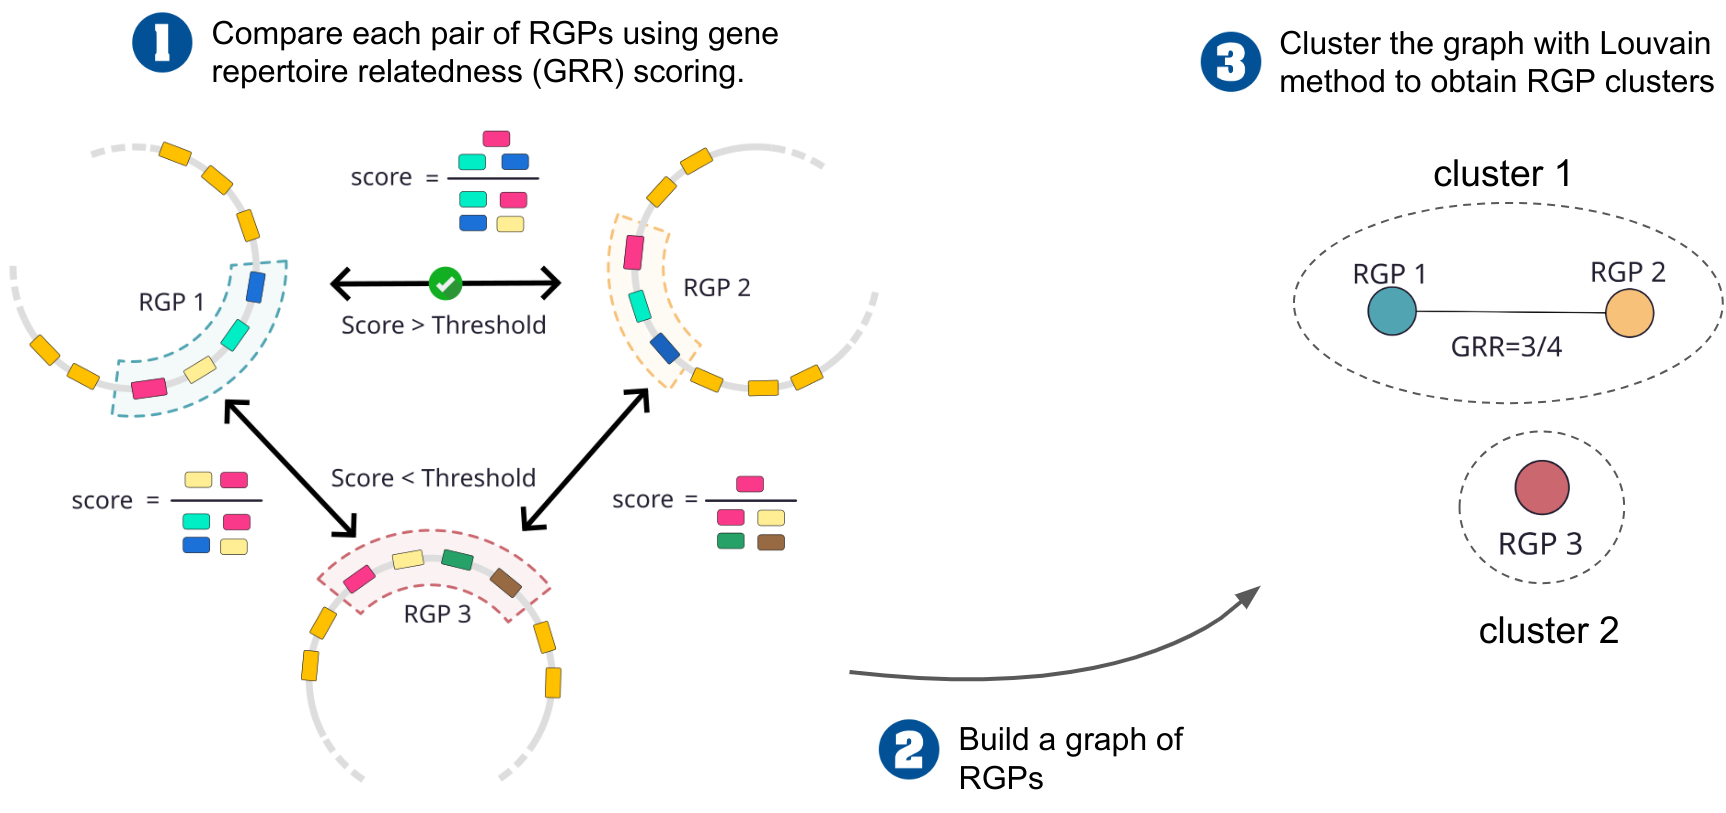
\includegraphics[width=\linewidth]{images/clusterRGPs.png}
    \label{fig:rgpcluster_met}}
    \hfill
    \subfloat[Application du clustering des RGPs sur le pangénome de \textit{A. baumannii} avec des métadonnées de résistance aux anitbiotiques (AMR)]{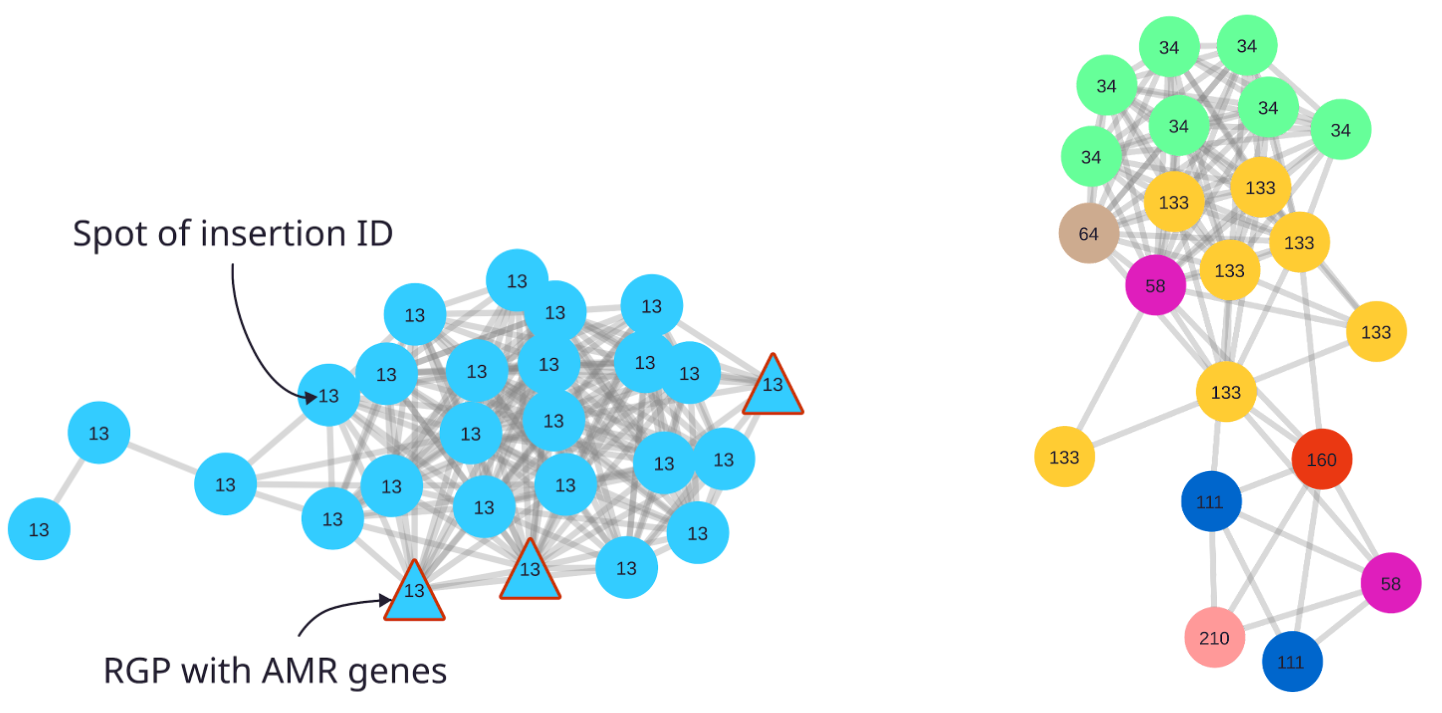
\includegraphics[width=\linewidth]{images/rgpclusterappli.png}
    \label{fig:rgpcluster_app}}
    \caption[Clustering des RGPs]{\textbf{Clustering des RGPs.}}
    \label{fig:rgpcluster}
\end{figure}

\subsection{Amélioration des procédures d'analyses}

\subsubsection{Lecture des fichiers d'annotation}

PPanGGOLiN permet la construction d'un graphe de pangénome à partir de séquences nucléiques et de génomes préalablement annotés. Les fichiers de génomes annotés (aux formats GFF ou GBFF) contiennent déjà les gènes ainsi que leurs coordonnées (contig, position, brin \dots). Ces fichiers peuvent également inclure des informations sur la fonction des gènes, des métadonnées relatives aux génomes et aux contigs, ainsi que la séquence des gènes ou des contigs eux-mêmes. Jusqu'à récemment, une partie de ces informations était ignorée par PPanGGOLiN. Désormais, elles sont lues et stockées dans le fichier de pangénome sous forme de métadonnées.

En nous intéressant à l'annotation fonctionnelle du pangénome, nous avons observé des divergences entre les séquences issues des fichiers d'annotation et celles correspondant aux gènes et aux familles de gènes. Nous avons notamment constaté que certaines coordonnées de gènes présentaient une complexité particulière et correspondaient à des événements biologiques spécifiques, tels que des décalages du cadre de lecture (\textit{frameshift}). Un ensemble de cas présentant des coordonnées atypiques a ainsi été identifié et est désormais correctement pris en charge dans PPanGGOLiN.

Ces améliorations ont conduit à une meilleure construction des familles de gènes, en corrigeant des séquences auparavant incorrectement tronquées ou décalées. Par ailleurs, elles ont permis d'améliorer la réécriture des séquences dans les fichiers de sortie, notamment ceux destinés à Proksee \cite{grant_proksee_2023}, et, par conséquent, la qualité des annotations fournies par les outils intégrés à cette plateforme.

\newpage

\subsubsection{Exécution de PPanGGOLiN via un fichier de configuration}

PPanGGOLiN intègre désormais la possibilité de générer un fichier de configuration. Ce fichier contient l’ensemble des commandes de PPanGGOLiN pouvant être exécutées ainsi que les paramètres spécifiques à chaque commande et les  globaux. A partir de ce fichier, PPanGGOLiN peut lancer une analyse \textit{de novo} sans préciser les paramètres de la ligne de commande. Ce fichier offre ainsi une alternative plus souple et organisée à l’exécution classique en ligne de commande. Il présente aussi plusieurs avantages.
(\textit{i}) Une exécution entièrement paramétrable des workflows. Jusqu’à présent, l’exécution de PPanGGOLiN dans un workflow reposait sur un nombre restreint de paramètres en ligne de commande. Cette limitation visait à éviter une surcharge des lignes de commande ainsi que d’éventuels conflits de nommage entre paramètres. Grâce aux fichiers de configuration, il devient possible de paramétrer entièrement un workflow, en définissant de manière explicite toutes les options requises. 
(\textit{ii}) Une intégration facilitée dans les pipelines d’analyse. L’utilisation de fichiers de configuration simplifie considérablement l’intégration de PPanGGOLiN dans des pipelines d’analyse. En effet, l’exécution d’outils en ligne de commande au sein de pipelines automatisés (souvent via des scripts Bash) peut poser plusieurs difficultés, telles que : une mauvaise interprétation des types de paramètres (par exemple, un entier lu comme une chaîne de caractères), des erreurs dans la gestion des chemins de fichiers, des conflits entre options spécifiques. L’emploi d’un fichier de configuration permet d’éliminer ces problèmes en standardisant et sécurisant la transmission des paramètres. Cette approche a notamment été adoptée lors de l’intégration de PPanGGOLiN dans MicroScope \cite{vallenet_microscope_2020}.

L’ajout des fichiers de configuration s’inscrit également dans les principes FAIR\footnote{Les principes FAIR visent à garantir que les données et les logiciels scientifiques soient faciles à retrouver (Findable), accessibles (Accessible), interopérables (Interoperable) et réutilisables (Reusable). Bien que ces principes aient été initialement conçus pour les données et le \textit{Big Data}, ils s’appliquent également aux outils bioinformatiques.}. En particulier, ils renforcent la reproductibilité des analyses. PPanGGOLiN permet ainsi de générer, à partir d’un pangénome, un fichier de configuration contenant toutes les options ayant permis sa construction. Cela garantit que, pour un même jeu de données, les analyses restent strictement reproductibles, favorisant ainsi une science plus ouverte et plus éthique. Cette avancée est particulièrement bénéfique dans un contexte de publication scientifique, où la transparence et la reproductibilité des analyses sont essentielles.

\newpage

\section{Optimisation technique}

Au-delà de l’ajout de nouvelles fonctionnalités, la version 2 de PPanGGOLiN a bénéficié de nombreuses améliorations visant à optimiser son efficacité, son ergonomie et sa maintenabilité. Parmi celles-ci, les optimisations techniques ont joué un rôle clé en réduisant la taille des fichiers générés, les temps de lecture ainsi que la mémoire utilisée.

\subsection{Amélioration de l'efficacité de PPanGGOLiN}

L’une des améliorations concerne l’optimisation du processus d’annotation des génomes. À cette fin, l’exécution de Prodigal \cite{hyatt_prodigal_2010} a été remplacée par l’intégration de Pyrodigal \cite{larralde_pyrodigal_2022}. Ce changement présente deux avantages principaux. 
Premièrement, la réduction des entrées/sorties (I/O) et l'amélioration de la gestion de la mémoire. Contrairement à l'exécution de Prodigal, qui nécessitait de générer des fichiers intermédiaires contenant les résultats d’annotation, Pyrodigal retourne directement les annotations sous forme d’objets Python utilisables par PPanGGOLiN. Cette approche permet de ne pas avoir à écrire et lire des fichiers intermédiaires pour chaque génome, réduisant ainsi l’empreinte mémoire et améliorant l’efficacité des opérations d’I/O. Deuxièmement, Pyrodigal intègre plusieurs améliorations au moteur de Prodigal, notamment une optimisation du calcul du score de connexion. Ce score est utilisé pour évaluer la probabilité d’une transition entre deux codons en fonction de divers critères (cadre de lecture, type de codon – initiation ou stop –, orientation du brin\dots). Comme l’a souligné Larralde \cite{larralde_pyrodigal_2022}, le calcul du score de connexion sur de longues séquences peut être coûteux en temps de calcul. Pyrodigal améliore ce processus en implémentant un filtrage heuristique, qui permet d’ignorer les connexions clairement invalides dès le départ. De plus, Pyrodigal exploite les fonctionnalités SIMD (Single Instruction, Multiple Data) des CPU modernes pour traiter plusieurs n\oe uds de calcul simultanément. Cela permet de traiter 8 n\oe uds avec les fonctionnalités NEON et SSE2, et 16 n\oe uds avec AVX2 (\autoref{fig:pyrodigal}). Ces optimisations réduisent le temps de calcul et améliorent significativement l’efficacité globale de la prédiction des gènes dans PPanGGOLiN.

\begin{figure}[htbp]
    \centering
    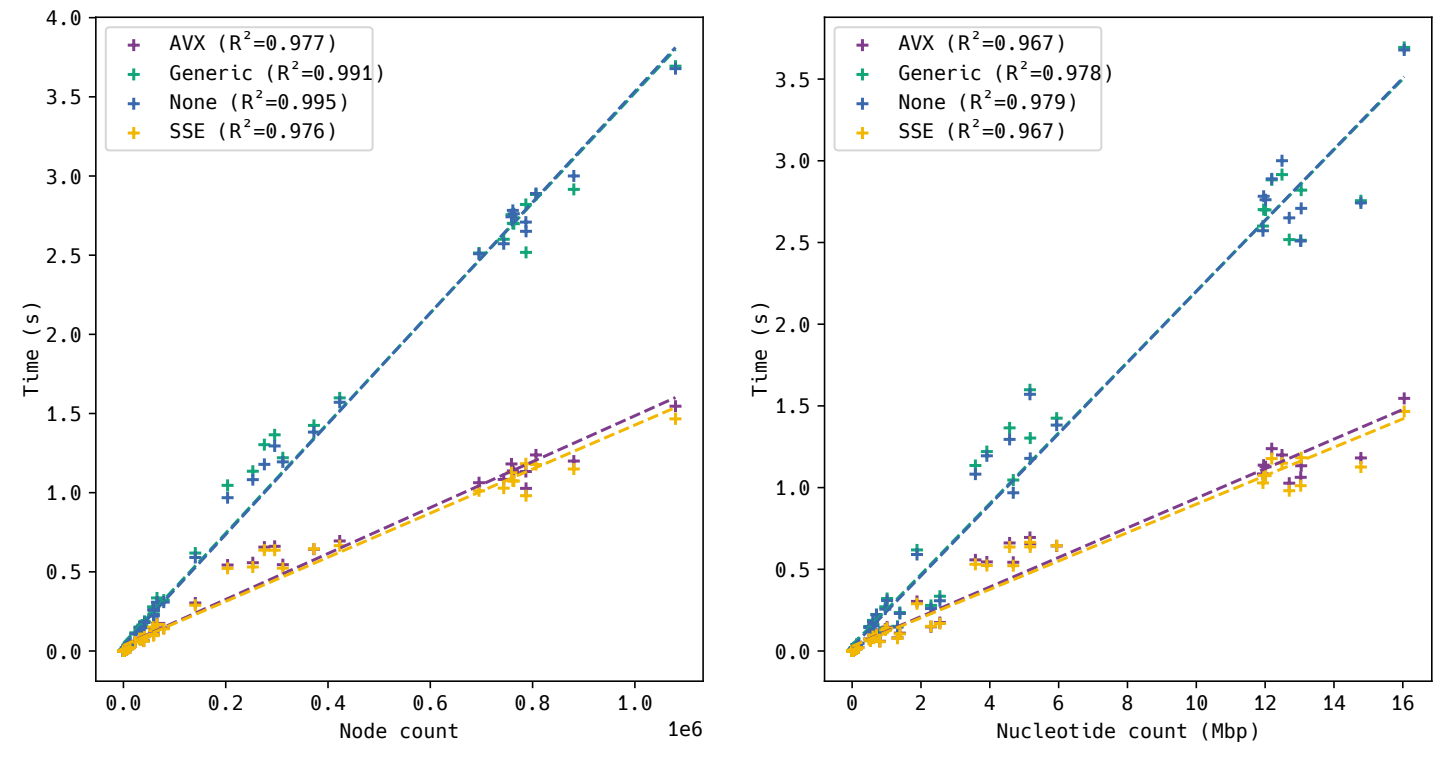
\includegraphics[width=0.8\linewidth]{images/pyrodigal.png}
    \caption[Évaluation des performances de calcul des scores de connexions]{\textbf{Évaluation des performances de calcul des scores de connexion.} L'évaluation est réalisé avec différents backends SIMD pour le filtre heuristique (SSE2 ou AVX2), avec un backend générique (\textit{Generic}) ou sans activer le filtre (\textit{None}). Chaque séquence a été traitée 10 fois sur un processeur \textit{i7-10710U} à 1,10 GHz. Extrait de \cite{larralde_pyrodigal_2022}}
    \label{fig:pyrodigal}
\end{figure}

Toujours dans l'objectif d'amélioration de l’efficacité de PPanGGOLiN, les fonctions de lecture ont été revues, afin de réduire le temps de chargement des données et l’utilisation de la mémoire. 
Pour atteindre cet objectif, plusieurs modifications ont été apportées à la manière dont les objets du pangénome sont interconnectés, afin de limiter le chargement de données inutiles. Dans PPanGGOLiN, la structure hiérarchique des objets implique, par exemple qu’un gène appartient à un contig, lequel est lui-même rattaché à un génome. Or, dans certaines commandes, le chargement des gènes entraînait systématiquement celui des contigs et des génomes, augmentant ainsi le temps d’exécution. Pour pallier ce problème, nous avons réorganisé ces dépendances et réécrit plusieurs fonctions de lecture afin de rendre l’accès aux données plus sélectif et plus efficace.

L’une des améliorations les plus significatives concerne la lecture des spots. Une réécriture de cette fonction a permis une réduction drastique du temps de lecture. Sur un pangénome de 3 083 génomes de \textit{E. coli}, le temps de lecture de 2 036 spots est passé de 25 minutes (dans un temps total de lecture du pangénome de 36 minutes) à seulement 3,5 secondes (pour un temps total réduit à 9 minutes et 38 secondes)\footnote{Cette amélioration est particulièrement visible sur les pangénomes de grande taille contenant un nombre important de spots, ce qui explique pourquoi le problème n’avait pas été détecté auparavant.}.

Dans cette même optique, des améliorations ont également été apportées à l’écriture des séquences (nucléotidiques et protéiques). Dans les versions précédentes de PPanGGOLiN, pour faciliter le filtrage des séquences demandées par l’utilisateur, l’ensemble du pangénome et de ses objets était chargé en mémoire, ce qui entraînait une consommation importante de ressources. Désormais, les séquences sont directement extraites du fichier HDF5, évitant ainsi la recréation systématique des objets du pangénome et réduisant significativement l’utilisation de la mémoire.

Avec l’augmentation continue du nombre de génomes disponibles, les pangénomes générés par PPanGGOLiN sont devenus de plus en plus volumineux. Malgré une structure de stockage compacte, reposant sur le package PyTable \cite{team_pytables_2002}, la taille des fichiers HDF5 a considérablement augmenté, en raison du nombre croissant de génomes et des nouvelles fonctionnalités enrichissant les données stockées.
Pour remédier à ce problème, l’architecture interne du fichier HDF5 a été revue afin d’éliminer les redondances, en particulier dans l’annotation des gènes et de leur séquence. En effet, entre différents génomes, les gènes peuvent partager des caractéristiques communes telles que leur position, leurs coordonnées ou encore leur orientation sur le brin. Or, ces informations étaient systématiquement dupliquées dans l’ancienne structure. Afin de réduire cette redondance, une table de référence a été mise en place pour centraliser ces informations et leur attribuer un identifiant unique, à la manière d’une base de données relationnelle. Chaque gène peut ainsi être associé à son annotation optimisée, sans nécessiter la répétition de ses caractéristiques dans l’ensemble du pangénome.
Cette optimisation a permis une réduction significative de la taille des fichiers HDF5. Comme illustré en \autoref{fig:ppanggoSize}, la taille des pangénomes a été divisée par 3,5 pour un ensemble de 1 000 génomes, et par 6,5 pour un pangénome de 2 500 génomes.
Au-delà du gain en espace de stockage, cette amélioration contribue également à l’accélération des temps de lecture. En effet, elle participe à la lecture non systématique des informations liées aux gènes lors du chargement du pangénome, ce qui allège le processus et améliore les performances globales de l’outil.

\begin{figure}
    \centering
    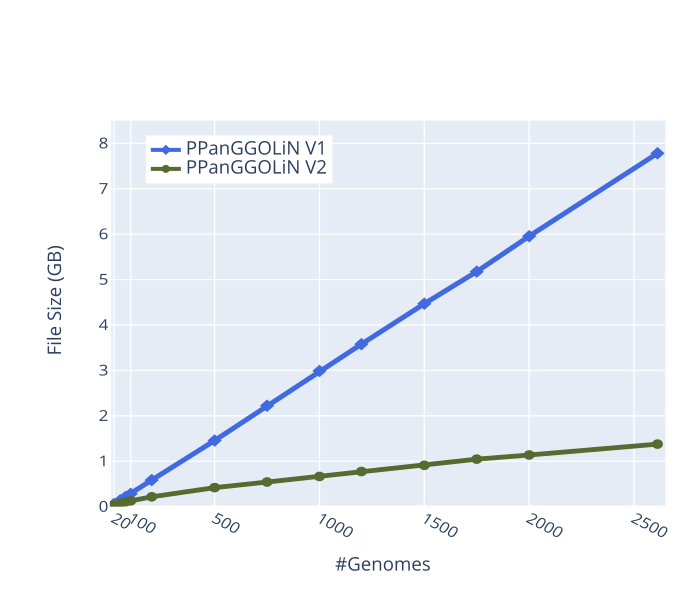
\includegraphics[width=.8\linewidth]{images/benchPPanGGO.png}
    \caption[Taille des fichiers de pangénome entre la version 1 et 2 de PPanGGOLiN]{\textbf{Comparaison des tailles des fichiers de pangénome entre la version 1 et 2 de PPanGGOLiN.}}
    \label{fig:ppanggoSize}
\end{figure}

Ces optimisations rendent PPanGGOLiN plus performant, plus rapide et plus adapté aux analyses pangénomiques de grande échelle, tout en maintenant une gestion efficace des ressources.

\subsection{Optimisation du code : lisibilité, maintenance, tests et processus de mise à jour}

En tant que logiciel open source, le code de PPanGGOLiN est accessible à tous, conformément aux principes de la science ouverte. Ce choix présente plusieurs avantages : il permet à la communauté d’utilisateurs de signaler d’éventuels comportements inattendus (problèmes de performance, bugs, \textit{etc}.), mais aussi de contribuer directement à l’amélioration du logiciel en proposant des corrections ou des optimisations.
Afin d’assurer la pérennité et la maintenabilité du projet, nous avons entrepris une révision complète du code, avec pour objectif principal de le rendre plus lisible, homogène et facile à maintenir pour les développeurs actuels et futurs.

\subsubsection{Mise en place de bonnes pratiques de développement}

La première étape du reformatage a consisté à aligner PPanGGOLiN avec les versions maintenues et corrigées de Python. Les packages les plus utilisés suivent également cette logique. En mettant à jour le code pour être compatible avec les versions récentes de Python, nous bénéficions des dernières mises à jour des packages, ainsi que des optimisations et corrections apportées par le langage lui-même. Ainsi, nous sommes passés de Python 3.8 à Python 3.12.

Pour améliorer la lisibilité et garantir une cohérence au sein du code, nous avons introduit un ensemble de règles et de processus applicables pour tous les développeurs. La première étape a été l’adoption des bonnes pratiques de codage en Python, en suivant les recommandations des PEP (\textit{Python Enhancement Proposals}).
L’application de ces directives présente plusieurs bénéfices. Premièrement, le code est plus structuré et lisible. Par exemple, les conventions de nommage permettent d’identifier rapidement la nature des variables et objets :

\begin{itemize}
    \item Nom des classes en CamelCase (\textit{e.g.} GeneCluster)
    \item Constantes en majuscules (\textit{e.g.} MAX\textunderscore ITERATIONS)
    \item Fonctions et méthodes en snake\textunderscore case (\textit{e.g.} compute\textunderscore similarity\textunderscore score)
\end{itemize}

Cette homogénéité facilite la lecture et la compréhension du code par tous les contributeurs. Deuxièmement, les règles PEP permettent de mettre en place des micro-optimisations pour de meilleures performances. Par exemple, en privilégiant l’utilisation de générateurs plutôt que des listes temporaires, ce qui permet d’optimiser l’utilisation de la mémoire.

Afin de faciliter l’application de ces règles et d’assurer leur respect de manière systématique, nous avons intégré le package python Black (\url{https://github.com/psf/black}) pour le formatage automatique du code. Lors de chaque mise à jour du code sur GitHub, Black est exécuté automatiquement pour reformater le code selon les standards des PEP. Cette automatisation garantit une cohérence stylistique, réduit la charge de travail des développeurs et simplifie la gestion des contributions extérieures.

Grâce à ces améliorations, le code de PPanGGOLiN devient plus clair, plus performant et plus facile à maintenir, assurant ainsi une plus grande longévité au projet et une meilleure collaboration au sein de la communauté open source.

\subsubsection{Maintenance et test du code}

PPanGGOLiN est avant tout un projet de recherche scientifique, ce qui implique des mises à jour fréquentes pour intégrer de nouvelles fonctionnalités et améliorer ses performances. Toutefois, ces modifications peuvent introduire des bogues susceptibles d’altérer la fiabilité des analyses. Afin de garantir la stabilité et la robustesse du logiciel, nous avons grandement amélioré la stratégie de tests automatisés, couvrant différents niveaux de validation.

\paragraph{Tests unitaires : validation des fonctionnalités élémentaires}

Les premiers tests mis en place sont des tests unitaires, qui permettent de vérifier le comportement individuel des fonctions. Ces tests s’assurent que chaque fonction produit bien le résultat attendu, et qu’elle génère les erreurs appropriées en cas d’entrée invalide. Actuellement, l'ensemble des classes sont testées et ainsi qu'une grande partie des fonctions.

\newpage

\paragraph{Tests d’intégration : validation des interactions entre fonctions}

Nous avons également mis en place des tests d'intégration, visant à évaluer le comportement global du logiciel lorsque plusieurs fonctions interagissent. En effet, une fonction peut répondre comme attendu de manière isolée tout en produisant des comportements imprévus lorsqu'elle est combinée à d'autres modules. Ces tests permettent donc de garantir la cohérence de l'ensemble du programme. Cependant, leur mise en \oe uvre reste complexe en raison des nombreuses interactions entre les fonctions dans PPanGGOLiN, ce qui limite la couverture de cette approche à une partie restreinte du code.

\paragraph{Tests fonctionnels : validation du comportement des commandes}

Enfin, nous avons introduit des tests fonctionnels, qui vérifient le comportement des commandes complètes. Pour cela, des fichiers de résultats de référence ont été préchargés, permettant de comparer automatiquement les nouvelles sorties avec les résultats attendus. Cette approche garantit que les évolutions du code n’altèrent pas l’exactitude des analyses produites par PPanGGOLiN. Toutes les commandes de PPanGGOLiN sont testées en prenant en compte tous les paramètres.


Lors d'une mise à jour du code, un workflow automatique est exécuté et permet de vérifier que le code est bien fonctionnel. Grâce à cette infrastructure de tests, le code est désormais plus robuste, limitant ainsi l’introduction de bogues imprévus et assurant la fiabilité des résultats scientifiques générés par le logiciel.

\subsubsection{Amélioration de l'expérience utilisateur}

PPanGGOLiN est un logiciel conçu pour les microbiologistes, dont l’expertise principale n’est pas nécessairement l’informatique. Il est donc essentiel de garantir une expérience utilisateur fluide, en facilitant aussi bien l’installation que l’utilisation du logiciel.

Un premier effort a été porté sur la réécriture complète de la documentation, afin de la rendre plus claire, plus structurée et mieux adaptée aux besoins des utilisateurs. Désormais, elle comprend :

\begin{itemize}
    \item Une section d’installation détaillant plusieurs méthodes adaptées à différents environnements,
    \item Un guide de prise en main rapide pour permettre aux utilisateurs d’exécuter rapidement PPanGGOLiN et ses principaux workflows,
    \item Des sections approfondies décrivant en détail chaque commande et analyse réalisable,
    \item Un guide dédié aux développeurs, recensant les bonnes pratiques et les processus de développement spécifiques à PPanGGOLiN.
\end{itemize}

De plus, la documentation est maintenant disponible sur ReadTheDocs, ce qui la rend plus accessible, mieux référencée et conforme aux principes FAIR.

\newpage

Un autre aspect clé de l’amélioration de l’expérience utilisateur concerne la gestion des erreurs. Afin de rendre les messages d’erreur plus explicites et plus informatifs, nous avons entrepris une révision complète de leur génération.
Les erreurs liées à une mauvaise utilisation par l’utilisateur sont maintenant décrites de manière plus claire et pédagogique. Les erreurs techniques, destinées aux développeurs, sont quant à elles plus précises, facilitant ainsi l’identification rapide de l’origine du problème. De plus, un plus large éventail de messages a été introduit pour couvrir davantage de cas d’erreur et améliorer la gestion des exceptions.


Grâce à ces améliorations, PPanGGOLiN devient plus intuitif pour les microbiologistes et plus facile à maintenir pour les développeurs, garantissant ainsi une expérience utilisateur optimisée.


